%\documentclass[11pt]{article}

% !TEX TS-program = pdflatex
% !TEX encoding = UTF-8 Unicode

% This is a simple template for a LaTeX document using the "article" class.
% See "book", "report", "letter" for other types of document.

\documentclass[11pt,a4paper]{report} % use larger type; default would be 10pt
%\documentclass[a4paper]{report}
\usepackage[utf8]{inputenc} % set input encoding (not needed with XeLaTeX)
\usepackage[francais]{babel}

\author{Gramaglia Alexis}

%%% Examples of Article customizations
% These packages are optional, depending whether you want the features they provide.
% See the LaTeX Companion or other references for full information.

%%% PAGE DIMENSIONS
\usepackage[T1]{fontenc}
\usepackage{geometry} % to change the page dimensions
\geometry{a4paper} % or letterpaper (US) or a5paper or....
%\usepackage{geometry}
 \geometry{
 a4paper,
 total={170mm,257mm},
 left=20mm,
 top=20mm,
 }
 \usepackage{xspace}
 
% \geometry{landscape} % set up the page for landscape%   read geometry.pdf for detailed page layout information
\usepackage{comment} % utiliser le commande comment pour commenter du code .tex
\usepackage{multicol}
\usepackage{wrapfig} % pour avoir une photo a cote du texte
\usepackage{graphicx} % support the \includegraphics command and options
\usepackage[parfill]{parskip} % Activate to begin paragraphs with an empty line rather than an indent
%%% PACKAGES
\usepackage{booktabs} % for much better looking tables
\usepackage{array} % for better arrays (eg matrices) in maths
\usepackage{paralist} % very flexible & customisable lists (eg. enumerate/itemize, etc.)
\usepackage{verbatim} % adds environment for commenting out blocks of text & for better verbatim
\usepackage{subfig} % make it possible to include more than one captioned figure/table in a single float
%\usepackage{mathabx}
%\usepackage{alltt}
\usepackage{listings}
\usepackage{color}
\usepackage{makeidx}
%\usepackage{stmaryrd}
\usepackage{caption}
\usepackage{xcolor}
\usepackage{hyperref}%avoir les liens actif
% These packages are all incorporated in the memoir class to one degree or another...

%%% HEADERS & FOOTERS
\usepackage{fancyhdr} % This should be set AFTER setting up the page geometry
\pagestyle{fancy} % options: empty , plain , fancy
\renewcommand{\headrulewidth}{0pt} % customise the layout...
\lhead{}\chead{}\rhead{}
\lfoot{}\cfoot{\thepage}\rfoot{}

%%%tableau
\usepackage{array,multirow,makecell}
%%%

%%% SECTION TITLE APPEARANCE
\usepackage{sectsty}
%\usepackage[Lenny]{fncychap}%Lenny,Rejne
\allsectionsfont{\sffamily\mdseries\upshape} % (See the fntguide.pdf for font help)

%%% ToC (table of contents) APPEARANCE
\usepackage[nottoc,notlof,notlot]{tocbibind} % Put the bibliography in the ToC
\usepackage[titles,subfigure]{tocloft} % Alter the style of the Table of Contents
\renewcommand{\cftsecfont}{\rmfamily\mdseries\upshape}
\renewcommand{\cftsecpagefont}{\rmfamily\mdseries\upshape} % No bold!

%%% END Article customizations

\usepackage{charter}%la police du document
\renewcommand{\headrulewidth}{0,1pt}
\fancyhead[C]{\leftmark}
\fancyhead[L]{}
\fancyhead[R]{}

%%%%%%%%%%%% MODIFICATION UD PIED DE PAGE %%%%%%%%%
\renewcommand{\footrulewidth}{1pt}
\fancyfoot[R]{\textbf{page\thepage}} 
\fancyfoot[L]{Gramaglia Alexis}
\fancyfoot[C]{}
%\fancyfoot[R]{\leftmark}
% -----------------------------------------------------



%-------------- CHANGER COULEUR SECTION,SUBSECTION ----------
\usepackage{titlesec}
%\titleformat*{\chapter}{\bfseries\color{green!40!black}}
%\titleformat*{\section}{\bfseries\color[rgb]{0.89,.0,.13}}
\titleformat*{\section}{\bfseries\color[rgb]{0.0,0.5,0.0}}
\titleformat*{\subsection}{\bfseries\color[rgb]{1.0, 0.49, 0.0}}
%\titleformat*{\subsubsection}{\bfseries\color{purple!40!black}}
\titleformat*{\subsubsection}{\bfseries\color[rgb]{.21,.46,.53}}
%--------------------------------------------------------------



\setlength{\parindent}{25pt} % pas d'indentation

%------------- Configuration table des matière -------------
\setcounter{secnumdepth}{2}
\setcounter{tocdepth}{1}
%--------------------------------------------------------------
\usepackage{hyperref}
\hypersetup{
pdfpagemode=UseOutlines,     % UseOutlines, UseThumbs, None, FullScreen : agencement au démarrage
pdfstartview=Fit,            % Fit, FitH, FitB, FitBH : vue de la page au départ (pleine largeur...)
pdffitwindow=true,           % bool: Maximiser
pdfpagelayout=TwoColumnsRight,% SinglePage, TwoColumnsRight/Left, OneColumn : affichage des pages
pdftoolbar=true,             % bool: Affichage de la barre d'outils
pdfmenubar=true,             % bool: Affichage de la barre de menus
bookmarksopen=false,         % bool: Dépliement des signets
bookmarksnumbered=true,      % bool: Numérotation des signets
colorlinks=true,             % bool: Liens colorés
pdfauthor={Gramaglia Alexis},         % Auteur	        % Titre
pdfcreator=PDFLaTeX,         % 
pdfproducer=PDFLaTeX,        %
linkcolor=black,              % Couleur des liens
urlcolor=black,               % url
anchorcolor=black,           % du texte
citecolor=black,             % Couleur de citation 
frenchlinks=true,            % bool: Utiliser des petites majuscules pour les liens, plutôt que de la couleur
pdfborder={0 0 0}             % Ne pas encadrer les liens
}


%---------- Pour pouvoir modifier la police du document ----- %
%\usepackage{helvet}
%\usepackage{tgadventor}
%\usepackage[T1]{fontenc}
%\usepackage{pxfonts} mettre la merde
%\renewcommand{\familydefault}{\sfdefault}
%--------------------------------------------------------------

%\usepackage{minted}% pour la coloration syntaxique
%\newminted[java]{java}{mathescape,linenos,frame=lines,breaklines,framesep=2mm}

\usepackage{tikz}

%------
\usetikzlibrary{backgrounds, calc, shadows, shadows.blur}






% Permet de gérer les numérotations dans la table des matières et dans le texte
\setcounter{secnumdepth}{4}

\definecolor{cas1}{RGB}{20, 107, 31}
\definecolor{cas2}{RGB}{122, 51, 193}
\definecolor{cas3}{RGB}{219, 16, 27}
\definecolor{cas4}{RGB}{209, 118, 20}
\definecolor{cas5}{RGB}{255, 0, 220}
\definecolor{cas6}{RGB}{141, 222, 9}
\definecolor{cas7}{RGB}{9, 127, 224}
\definecolor{cas8}{RGB}{38, 22, 249}
\definecolor{cas6bis}{RGB}{118, 0, 57}

\definecolor{blueDWord}{rgb}{0, 0.09,0.58}
\definecolor{blueWord}{rgb}{0.16, 0.34, 0.63}
\definecolor{greenWord}{rgb}{0.54, 0.72, 0.22}
\definecolor{redWord}{rgb}{0.71, 0.15, 0.17}
\definecolor{violetWord}{rgb}{0.39, 0.25, 0.57}
\definecolor{orangeWord}{rgb}{0.91, 0.44, 0.12}
\definecolor{pinkWord}{rgb}{1, 0.25,1}
\definecolor{powderblue}{rgb}{0.69, 0.88, 0.9}
\definecolor{green}{RGB}{0, 153, 0}

\definecolor{mauve}{rgb}{149, 0, 187}


\usepackage{longtable}


% oNE PAGE SINGLE HORIZONTALE
\usepackage{lscape}

\usepackage{wrapfig}

%tableau long
\usepackage{fourier}
\usepackage{longtable}

% figure H
\usepackage{float}

%http://tex.stackexchange.com/questions/41247/add-pdf-bookmark-manually
%\usepackage[bookmarks=true]{hyperref}
\usepackage{bookmark}

% 3 images 
%http://tex.stackexchange.com/questions/64858/how-to-create-subfloat-figures-two-in-first-row-and-one-below
\usepackage{subfig}


% Pour encadrer les formules
%http://tex.stackexchange.com/questions/122945/coloured-shadowed-boxes-around-equations
\usepackage[skins,theorems]{tcolorbox}
\tcbset{highlight math style={enhanced,
  colframe=red,colback=white,arc=0pt,boxrule=1pt}}

  
  
\usepackage[framemethod=tikz]{mdframed}
  
 %pour les equations
 \usepackage{amsmath}
\usepackage{amsfonts}
\usepackage{amssymb}
  
 % barrer le texte
 \usepackage{cancel}
 
 \usepackage[squaren, Gray, cdot]{SIunits}


 
\setlength\parindent{0pt}

\usepackage[skins,theorems]{tcolorbox}
\tcbset{highlight math style={enhanced,
  colframe=red,colback=white,arc=0pt,boxrule=1pt}}
\newmdenv[innerlinewidth=0.5pt, ,linecolor=red,innerleftmargin=6pt,
innerrightmargin=6pt,innertopmargin=6pt,innerbottommargin=6pt]{mybox}








%========================================
% Constantes de configuration du document
%========================================

%----------------------------------
% Identité de l'école
%----------------------------------
\newcommand{\ecole}{Institut Supérieur Industriel de Bruxelles}
\newcommand{\entite}{Haute école Paul-Henri Spaak}
\newcommand{\entiteadresse}{Rue Royale, 150. 1000 Bruxelles}
\newcommand{\entitesite}{http://www.isib.be}
\newcommand{\entitetel}{02/217.46.09}
\newcommand{\entitemail}{isib@isib.be}
\newcommand{\etude}{Ingénieur industriel en informatique}


% ----------------------------------
% Identité de l'AA
% ----------------------------------
\renewcommand{\aa}{LABO_ELEC}
\newcommand{\cours}{Laboratoire d'électronique appliquée}
\newcommand{\titre}{Rapport}
\newcommand{\prof}{Mme. Degeest}
% ----------------------------------
% Information sur l'auteur
% ----------------------------------
\newcommand{\auteur}{Maeck Jeremy \& Gramaglia Alexis}
\newcommand{\annee}{2016-2017}
\newcommand{\anneeEtude}{Ingénieur industriel en informatique - année passerelle }
\newcommand{\sectionEtude}{Finalité : \textit{Ingénieur industriel en informatique }}
\newcommand{\dateedition}{\today}
\title{Rapport }
\begin{document}
% =========================================================
% 1ère page du syllabus
% Utilise des constantes définies dans le fichier de config
% =========================================================

\thispagestyle{empty}

%----------------------------------
% haut : logo + infos écoles
%----------------------------------

\includegraphics[scale=0.8]{ressources/isib-logo.png}
\quad
\begin{minipage}[t]{7cm}
	\vspace{-7\baselineskip}
	\sffamily\large
	\textbf{\ecole\\\entite\\\etude}
	\bigskip\\
	\entiteadresse\\\entitetel{} – \entitemail
\end{minipage}

%----------------------------------
% centre : cours, anneeEtude, section
%----------------------------------
\vfill
\begin{center}
	\sffamily
	\Huge\cours
	\bigskip\\
	\Large\titre
	\bigskip\\
	%\Large\anneeEtude
	%\bigskip\\
	\Large\sectionEtude
	\bigskip\\
	\Large\prof
\end{center}
\vfill

%----------------------------------
% bas : auteur,annee
%----------------------------------
\begin{center}
	\Large\auteur\\
	\Large\annee
\end{center}

\chapter{Objectif \& description} 

L'objectif de ce projet était de réaliser un circuit électronique du début à la fin. Nous avons commencé par choisir un sujet et avons opté pour un détecteur de sonnerie réveil. Ce circuit électronique allait donc être capable de détecter une sonnerie et faire clignoter une LED au même rythme. Nous avons ensuite du concevoir le schéma du circuit grâce au logiciel Eagle, le tester sur breadboard pour enfin pouvoir le réaliser sur une carte imprimée.

\section{Sujet initial}

Le sujet initial consistait donc à détecter la sonnerie d'un réveil. Le schéma du circuit que nous avions récupéré utilisait donc un réveil. Voici le schéma : 

\begin{figure}[H]
\centering
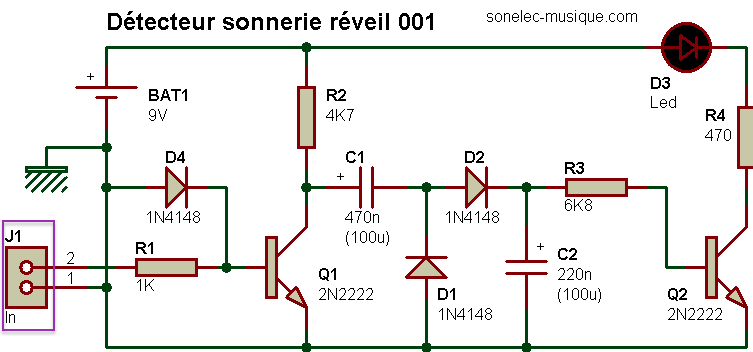
\includegraphics[width=1\textwidth]{ressources/schema_initTransdu}
\caption{Schéma initial}
\label{schemaInit}
\end{figure}

Nous pouvons observé que ce circuit est relié au transducteur (élement encadré) du réveil. Cet élément permet de transformer en ondes sonores les impulsions électriques venant du réveil. Le principe initial était donc d'aller récupérer ces impulsions électriques sur le transducteur afin de pouvoir allumer la LED. 
N'ayant pas de réveil en notre possession nous avons décidé d'opter pour une solution alternative dans laquelle nous n'avions pas besoin du transducteur. L'idée était de remplacer le réveil par un buzzer.

\chapter{Test du circuit sur breadboard}

Lorsque notre choix fut confirmé, nous avons du tester le circuit choisi sur une breadboard afin de valider le bon fonctionnement de celui-ci. 

Nous avons donc commencé par nous procurer les différents composants dont on avait besoin. Ensuite nous avons reproduit le schéma initial sur la breadboard.

Lorsque que cette étape fut terminée, nous avons testé le circuit. Malheureusement un problème c'est présenté. En effet, l'idée que nous avions de remplacer le transducteur par un simple buzzer n'était pas aboutie parfaitement. 

Nous avons donc cherché la provenance du problème et après réflexion nous en sommes venus à la conclusion suivante. Afin que le buzzer puisse remplacer correctement le transducteur du réveil, celui-ci devait se voir fournir une alimentation supplémentaire à celle fournie au circuit électrique. Pour que le buzzer ne soit pas activé en permanence, nous avons également ajouté un interrupteur entre l'alimentation et le buzzer. Voici le circuit final réalisé sur la breadboard : 

\begin{figure}[H]
\centering
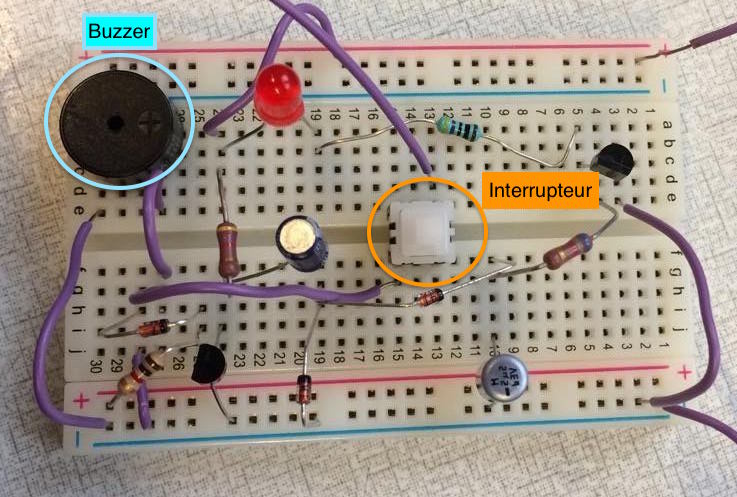
\includegraphics[width=0.7\textwidth]{ressources/breadboardElement}
\caption{Circuit sur breadboard}
\end{figure}

\chapter{Conception du schéma}

Afin de concevoir le schéma électronique de notre circuit nous avons utilisé le logiciel Eagle. Nous avons donc commencé par prendre en main ce logiciel et ensuite créé le schéma.  

Etant donné que Eagle nous produira le schéma qui sera imprimé sur la carte, il était donc important de choisir les bons composants. Ce n'était pas à la caractéristique intrinséque des composants qu'il fallait faire attention mais bien à la dimension de ceux-ci . Nous avons donc créé le schéma de notre circuit électrique en prenant en compte les dimensions de chaque composants. Voici le schéma que nous avons réalisé : 


\begin{figure}[H]
\centering
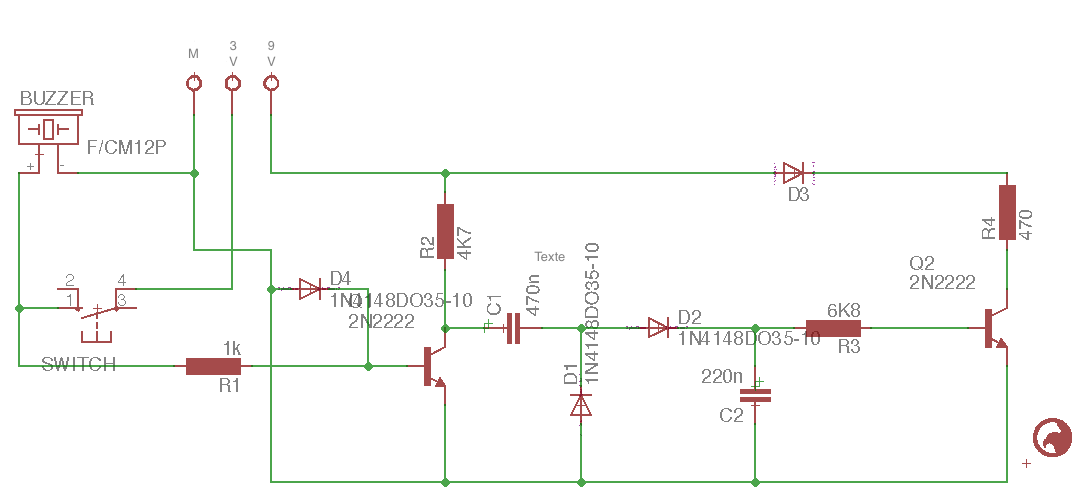
\includegraphics[width=1\textwidth]{ressources/schema_final}
\caption{Schéma avec buzzer}
\label{schemaEagle}
\end{figure}

Comme indiqué sur la figure \ref{schemaEagle}, pour réaliser ce circuit il nous a fallut :
\begin{itemize}
	\item une capacité de \textbf{$470 nF$}
	\item une capacité de \textbf{$220 nF$}
	\item 3 diode $1N4148$
	\item une résistance de $ 1k\ohm $
	\item  une résistance de $ 4,7K\ohm $
	\item  une résistance de $ 6,8K\ohm $
	\item une résistance de $470\ohm $
\end{itemize}



\end{document}



